\documentclass[12pt]{article}
\usepackage{amsmath}
\usepackage{amssymb}
\usepackage{tikz}
\usepackage{pgfplots}
\usepackage{float}
\begin{document}
\title{Electrical Engineering 102, Homework 2}
\date{October 17th, 2018}
\author{Michael Wu\\UID: 404751542}
\maketitle

\section*{Problem 1}

\paragraph{a)}

\begin{enumerate}
	\item \(x(t)(u(t-1)-u(2t-3))\)
	\begin{center}
		\begin{tikzpicture}[scale=0.8]
			\begin{axis}[ymin=-1.2,ymax=1.2,xmax=2.99,xmin=-2.99,axis lines = middle]
				\addplot[color=black,mark=none] coordinates {
					(1,0)
					(1,0.25)
					(1.5,0.375)
					(1.5,0)
				};
			\end{axis}
		\end{tikzpicture}
	\end{center}
	\item This simplifies to \(x(t)(1+\delta(t-1))\).
	\begin{center}
		\begin{tikzpicture}[scale=0.7]
			\begin{axis}[ymin=0,ymax=1.19,xmax=4.99,xmin=0,axis lines = middle]
				\addplot[color=black,mark=none] coordinates {
					(0,0)
					(1,0.25)
					(1,1)
					(1,0.25)
					(4,1)
					(4,0)
				};
			\end{axis}
		\end{tikzpicture}
	\end{center}
	\item \(\frac{d}{dt}x(t)\)
	\begin{center}
		\begin{tikzpicture}[scale=0.7]
			\begin{axis}[ymin=0,ymax=1.19,xmax=4.99,xmin=0,axis lines = middle]
				\addplot[color=black,mark=none] coordinates {
					(0,0)
					(0,0.25)
					(4,0.25)
					(4,0)
				};
			\end{axis}
		\end{tikzpicture}
	\end{center}
	\item \(x(t)-\frac{1}{2}r(t)+\frac{1}{2}r(t-4)+2u(t-4)\)
	\begin{center}
		\begin{tikzpicture}[scale=0.7]
			\begin{axis}[ymin=-1.19,ymax=0,xmax=4.99,xmin=0,
				axis y line = middle,
				y axis line style = {stealth-},
				axis x line = top]
				\addplot[color=black,mark=none] coordinates {
					(0,0)
					(4,-1)
					(4,0)
				};
			\end{axis}
		\end{tikzpicture}
	\end{center}
\end{enumerate}

\paragraph{b)}

\begin{enumerate}
	\item \(f(0)\)
	\item
	\(\begin{cases}
		\frac{1}{2e^2} & t\leq1\\
		\frac{1}{2e^{2t}} & t>1
	\end{cases}\)
	\item \(f(1)\)
	\item \(f(2)\delta(t-2)\)
\end{enumerate}

\paragraph{c)}

We have that
\[\delta(bt)=\lim_{\Delta\to 0} \text{rect}_{\Delta}(bt)\]
and
\[
	\text{rect}_{\Delta}(t)=
	\begin{cases}
		\frac{1}{\Delta} & |t|\leq\frac{\Delta}{2}\\
		0 & \text{else}
	\end{cases}
\]
Thus we get
\begin{align*}
	\text{rect}_{\Delta}(bt)&=
	\begin{cases}
		\frac{1}{\Delta} & |bt|\leq\frac{\Delta}{2}\\
		0 & \text{else}
	\end{cases}\\
	&=
	\begin{cases}
		\frac{1}{\Delta} & |t|\leq\frac{\Delta}{2b}\\
		0 & \text{else}
	\end{cases}\\
	&=
	\begin{cases}
		\frac{1}{bu} & |t|\leq\frac{u}{2}\\
		0 & \text{else}
	\end{cases}\\
	&=
	\frac{1}{b}
	\begin{cases}
		\frac{1}{u} & |t|\leq\frac{u}{2}\\
		0 & \text{else}
	\end{cases}\\
	&=\frac{1}{b}\text{rect}_u(t)
\end{align*}
where \(u=\frac{\Delta}{b}\). Therefore
\[\delta(bt)=\frac{1}{b}\lim_{u\to 0} \text{rect}_{u}(t)=\frac{1}{b}\delta(t)\]

\section*{Problem 2}

\paragraph{a)}

\begin{enumerate}
	\item \(\frac{3}{2}\Delta(t-1) + \Delta(t-2)\)
	\item \(\text{rect}(t)+\Delta(t-1)+\Delta(t+1)\)
	\item \(2(\Delta(2t)+\Delta(2t-2)+\Delta(2t+2))+\Delta(2t-3)+\Delta(2t+3)\)
\end{enumerate}

\paragraph{b)}

\begin{enumerate}
	\item \(x_a(t)=u(t+2)+\frac{1}{2}u(t+1)-2u(2t-3)+\frac{1}{2}u(t-3)\)
	\item \(x_b(t)=\frac{3}{2}u(t+1)-\frac{5}{2}u(t)+u(t-1)\)
\end{enumerate}

\section*{Problem 3}

\paragraph{a)}

\begin{enumerate}
	\item This system is not time-invariant, not causal, and stable. It is not time-invariant because of the \(2t\) term, which makes a delay on the input not directly correspond to a delay in the output.
	It is not causal because the \(2t\) term may require looking into the future. For example if \(t=2\) we must evaluate \(x(4)\). It is stable because at most the signal \(|y(t)|\) is bounded by
	\(2\max(|x(t)|)\).
	\item This system is time-invariant, not causal, and stable. It is time invariant because it is essentially the area under the input signal within a certain interval. So delaying the input signal will result
	in a directly corresponding delay in the output signal, as the whole integral will be shifted over. It is not causal because the \(t+T\) term requires looking into the future. It is stable because
	the output signal \(|y(t)|\) is bounded by \(2T\max(|x(t)|)\).
	\item This system is not time-invariant, causal, and not stable. It is not time-invariant because of the \(t+1\) term, which will change over time regardless of a delay on the input. It is causal
	because there is no need to evaluate the input signal at any point in the future. It is not stable because the lower limit of integration is infinite. Thus the integral may not converge even if the input
	is bounded.
	\item This system is not time-invariant, causal, and stable. It is not time-invariant because the \(\cos(\omega t)\) term will not be delayed if the input is delayed, resulting in a differently shaped
	output signal if there is a delay in the input. It is causal because it only requires evaluating \(x(t)\), which is in the present. It is stable because the cosine term is bounded by \(-1\) and \(1\),
	so \(|y(t)|\) is bounded by \(1+\max(|x(t)|)\).
	\item This system is not time-invariant, causal, and stable. Consider \(x(t)=-\omega t\), which results in the output signal being a constant at \(1\). If the input was \(x(t-1)\), the output would then be a
	constant at \(\cos(\omega)\), so the signal is not time-invariant because it changes shaped due to a delay in the input signal. It is causal because the system only evaluates \(x(t)\) at the present. It is
	stable because the cosine term is bounded by \(-1\) and \(1\).
	\item This system is not time-invariant, not causal, and not stable. It is not time-invariant because of the \(\frac{t}{2}\) term. It is also not causal because the \(\frac{t}{2}\) term would require looking
	into the future when \(t<0\). It is not stable because the lower limit of the integral is \(-\infty\), so a bounded input such as the constant \(x(t)=1\) may result in an infinite output.
	\item This system is time-invariant, causal, and stable. It is time invariant because the time component only shows up in \(x(t)\), so a delay in the input signal directly corresponds to a delay in the output signal.
	It is also causal because the output signal only depends on the current value of the input signal. It is stable because \(1+x^2(t)\) must be greater than \(1\), assuming \(x(t)\) is real. This results in an output that
	must be between \(0\) and \(1\).
\end{enumerate}

\paragraph{b)}

Our system is given by the equation
\[\frac{x(t)+x(-t)}{2}\]
This means that the signal is not time invariant, delaying \(x(t)\) would not result in a corresponding delay in the output signal. This is because the even part must be symmetrical about the origin, so
it would change shape instead of being delayed. It is stable because at most the output is bounded by the maximum value of \(x(t)\).

\paragraph{c)}

First let us evaluate \(z(t)\) in terms of \(x(t)\).
\[z(t)=\int_{-\infty}^t x\left(\frac{\tau}{2}\right)\,d\tau = 2\int_{-\infty}^{\frac{t}{2}}x(u)\,du\]
Here we have made the substitution \(u=\frac{\tau}{2}\). If we choose \(S_3\) to be given by \(y(t)=\frac{1}{2}z(2t-2)\), we
then obtain the desired result of
\[y(t)=\int_{-\infty}^{t-1}x(\tau)\,d\tau\]

\pagebreak

\paragraph{d)}

\begin{enumerate}
	\item We have that \(z(t-\delta)=S_1(x(t-\delta))\) for all \(\delta\). We also have that \(y(t-\delta)=S_2(z(t-\delta))\) for all \(\delta\).
	Using substitution, this results in
	\[y(t-\delta)=S_2(S_1(x(t-\delta)))\]
	for all \(\delta\). This means that the series cascade of any two time-invariant systems is also time invariant.
	\item We have that \(y_1(t-\delta)=S_1(x(t-\delta))\) for all \(\delta\). We also have that \(y_2(t-\delta)=S_2(x(t-\delta))\) for all \(\delta\).
	Finally we have that \(y(t)=y_1(t)+y_2(t)\). Then we get
	\[y(t-\delta)=y_1(t-\delta)+y_2(t-\delta)=S_1(x(t-\delta))+S_2(x(t-\delta))\]
	for all \(\delta\). Therefore the parallel cascade of any two time-invariant systems is also time invariant.
	\item Consider the two time-variant systems \(y(t)=x(2t)\) and \(y(t)=x\left(\frac{t}{2}\right)\). Their series cascade is equivalent to \(y(t)=x(t)\), which is time-invariant.
	Consider the two time-variant systems which are the even and odd components of a signal. Added together they result in the original signal, which is equivalent
	to the system \(y(t)=x(t)\). Thus their parallel cascade is time-invariant.
\end{enumerate}

\section*{Problem 4}

\paragraph{a)}

As this signal is periodic, it must be a power signal. We then evaluate its power as follows.
\begin{align*}
	P&=\lim_{T\to\infty} \frac{1}{2T}\int_{-T}^T |x(t)|^2\,dt\\
	&=\lim_{T\to\infty} \frac{1}{2T}\int_{-T}^T (Ae^{j\omega t}+Be^{-j\omega t})(Ae^{-j\omega t}+Be^{j\omega t})\,dt\\
	&=\lim_{T\to\infty} \frac{1}{2T}\int_{-T}^T (A^2+AB(e^{j2\omega t}+e^{-j2\omega t})+B^2)\,dt\\
	&=\lim_{T\to\infty} \frac{1}{2T}\int_{-T}^T (A^2+2AB\cos(2\omega t)+B^2)\,dt\\
	&=\lim_{T\to\infty} \frac{1}{2T}\left.(A^2+B^2)t + \frac{AB}{\omega}\sin(2\omega t)\right|_{-T}^T\\
	&=\lim_{T\to\infty} \frac{(A^2+B^2)2T+\frac{2AB}{\omega}\sin(2\omega T)}{2T}\\
	&=A^2+B^2
\end{align*}

\paragraph{b)}

Due to the decaying term it is an energy signal. We then evaluate its energy as follows.
\begin{align*}
	E&=\int_{-\infty}^\infty |x(t)|^2\,dt\\
	&=\int_{-\infty}^\infty |e^{-(1+j\omega)t}u(t-1)|^2\,dt\\
	&=\int_1^\infty |e^{-t}e^{-j\omega t}|^2\,dt\\
	&=\int_1^\infty e^{-2t}\,dt\\
	&=\left. -\frac{e^{-2t}}{2}\right|_1^\infty\\
	&=\frac{1}{2e^2}
\end{align*}

\section*{Problem 5}

\paragraph{a)}

I generated the plot using the following code.
\begin{verbatim}
t=linspace(0,10,500);
y=exp((-log(2)/10+1i*pi).*t);
plot(y);
set(gcf,'color','w');
export_fig problem5a.pdf;
\end{verbatim}
I chose \(\sigma=-\frac{\ln(2)}{10}\) and \(\omega=\pi\).
\begin{figure}[H]
    \begin{center}
        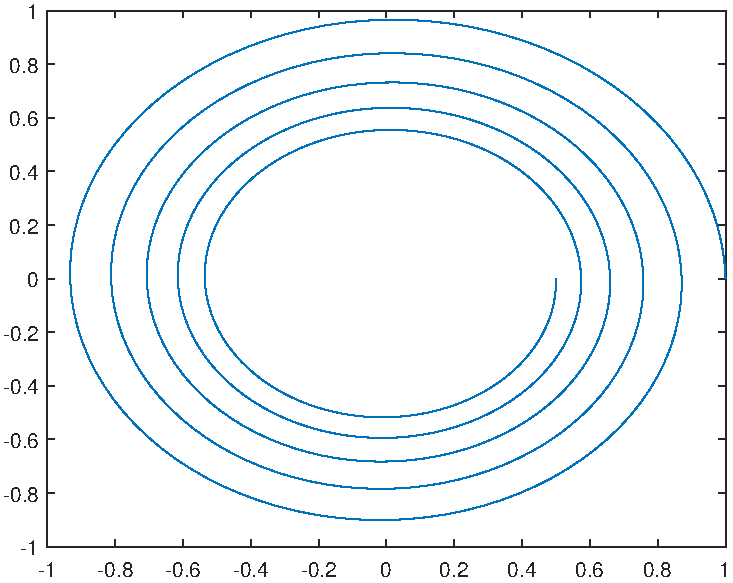
\includegraphics[width=2.5in]{problem5a.pdf}
    \end{center}
\end{figure}
Here MATLAB is plotting the real component of the signal on the \(x\) axis and the imaginary component on the \(y\) axis.

\paragraph{b)}

I generated the plots using the following code.
\begin{verbatim}
t=linspace(0,10,500);
y=exp((-log(2)/10+1i*pi).*t);
plot(t,real(y));
set(gcf,'color','w');
ylabel('real(y(t))');
xlabel('t(sec)');
export_fig problem5b-real.pdf;
plot(t,imag(y));
ylabel('imag(y(t))');
xlabel('t(sec)');
export_fig problem5b-imag.pdf;
\end{verbatim}
\begin{figure}[H]
    \begin{center}
        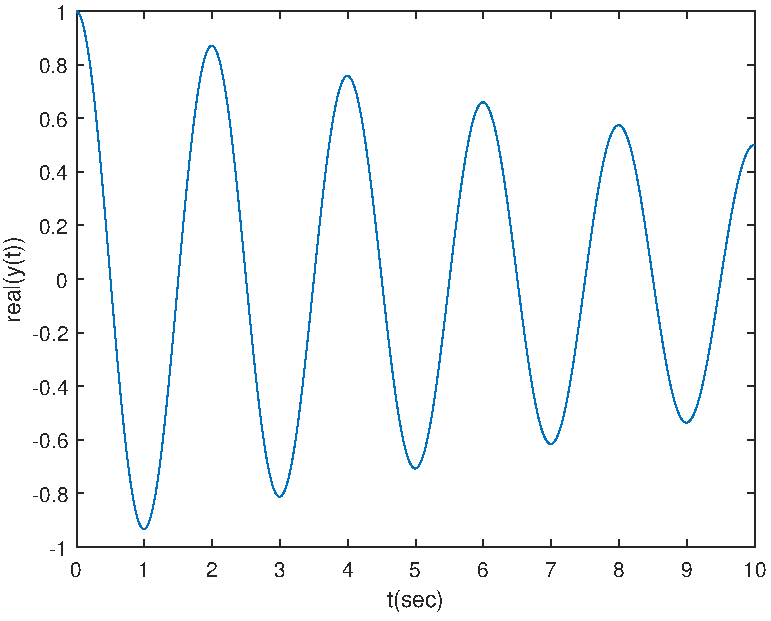
\includegraphics[width=2.5in]{problem5b-real.pdf}
		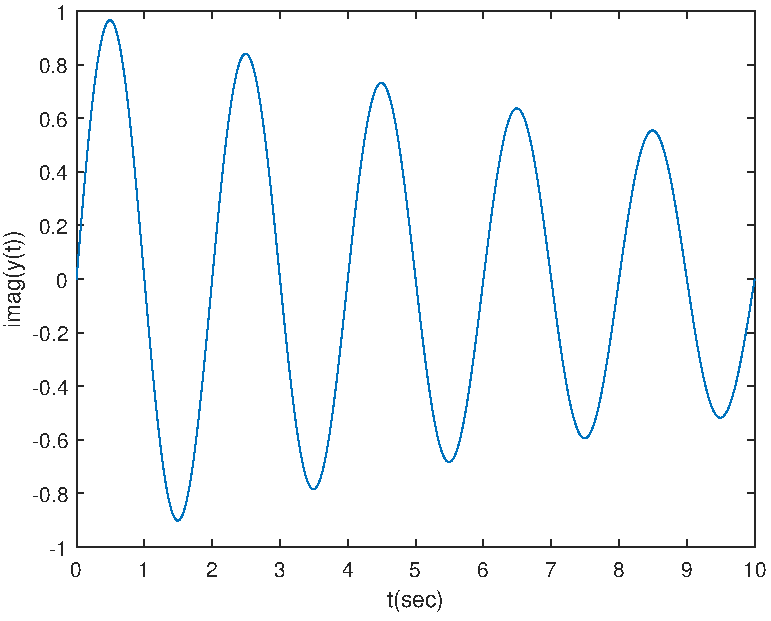
\includegraphics[width=2.5in]{problem5b-imag.pdf}
    \end{center}
\end{figure}

\paragraph{c)}

I generated the plot using the following code.
\begin{verbatim}
t=linspace(0,10,500);
y=exp((-log(2)/10+1i*pi).*t);
plot(t,abs(y));
hold on
plot(t,wrapTo2Pi(angle(y))/(2*pi));
hold off
set(gcf,'color','w');
xlabel('t(sec)');
export_fig problem5c.pdf;
\end{verbatim}
Here the blue line is the magnitude and the red line is the phase angle in terms of cycles.
\begin{figure}[H]
    \begin{center}
        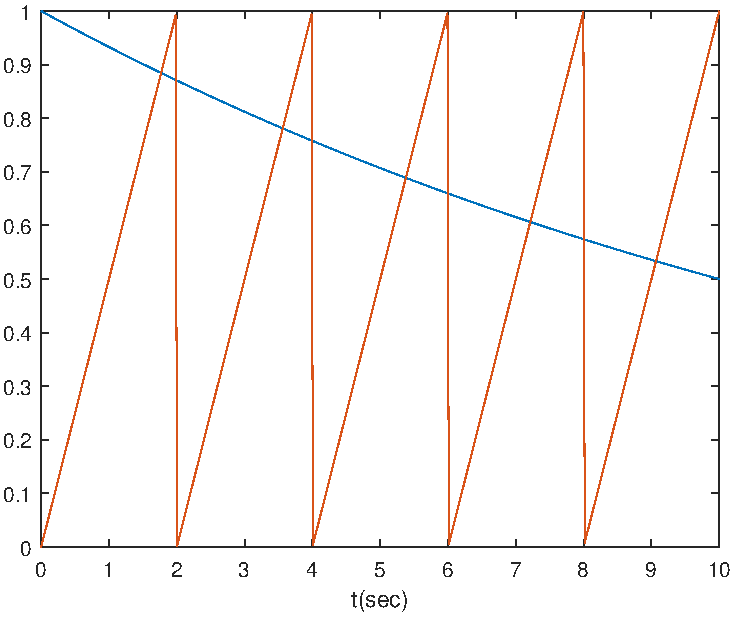
\includegraphics[width=2.5in]{problem5c.pdf}
    \end{center}
\end{figure}

\end{document}